\documentclass{article}

% content/resources/templates/preamble.tex
\usepackage[margin=0.6in]{geometry}
\author{Milav Dabgar}
\usepackage{amsmath,amssymb,amsthm}
\usepackage{booktabs}
\usepackage{multirow}
\usepackage{xcolor}
\usepackage{tcolorbox}
\tcbuselibrary{breakable,skins}
\usepackage[colorlinks=true,linkcolor=blue]{hyperref}
\usepackage{titlesec}
\usepackage{enumitem}
\usepackage{tikz}
\usepackage{pgfplots}
\usepackage{circuitikz}
\usepackage[version=4]{mhchem}
\usepackage{longtable}
\usepackage{array}
\usepackage{float}
\usepackage{caption}
\usepackage{listings}

\lstset{
  basicstyle=\small\ttfamily,
  breaklines=true,
  breakatwhitespace=false,
  postbreak=\mbox{\textcolor{red}{$\hookrightarrow$}\space},
  float=false,
  numbers=left,
  numberstyle=\tiny\color{gray},
  numbersep=10pt,
  xleftmargin=2em,
  keywordstyle=\color{blue},
  commentstyle=\color{green!60!black},
  stringstyle=\color{purple},
  backgroundcolor=\color{gray!5},
  showstringspaces=false,
  tabsize=2,
  captionpos=b,
  keepspaces=true,
  columns=flexible
}

\pgfplotsset{compat=1.18}
\usetikzlibrary{shapes,arrows,positioning,calc,patterns,decorations.pathmorphing,decorations.markings,arrows.meta}

% Color scheme
\definecolor{headcolor}{RGB}{0,102,204}
\definecolor{keycolor}{RGB}{220,20,60}
\definecolor{solutioncolor}{RGB}{34,139,34}
\definecolor{mnemoniccolor}{RGB}{148,0,211}
\definecolor{codecolor}{RGB}{0,0,100}

% Spacing
\setlength{\parskip}{3pt}
\setlist[itemize]{nosep}
\setlist[enumerate]{nosep}

% Title formatting
\titleformat{\section}{\Large\bfseries\color{headcolor}}{\thesection}{1em}{}
\titleformat{\subsection}{\large\bfseries\color{headcolor}}{\thesubsection}{1em}{}

% Pandoc tightlist compatibility
\providecommand{\tightlist}{%
  \setlength{\itemsep}{0pt}\setlength{\parskip}{0pt}}

% Pandoc longtable compatibility
\newcounter{none}
\def\thenone{}


% content/resources/templates/english-boxes.tex

% Custom environments
\newtcolorbox{solutionbox}{
 breakable,
 enhanced,
 colback=solutioncolor!5!white,
 colframe=solutioncolor!75!black,
 fonttitle=\bfseries,
 title=Solution
}

\newtcolorbox{solutionboxnobreak}{
 colback=solutioncolor!5!white,
 colframe=solutioncolor!75!black,
 fonttitle=\bfseries,
 title=Solution
}

\newtcolorbox{keyformula}{
 breakable,
 enhanced,
 colback=keycolor!5!white,
 colframe=keycolor!75!black,
 fonttitle=\bfseries,
 title=Key Formula
}

\newtcolorbox{mnemonicboxenv}{
 breakable,
 enhanced,
 colback=mnemoniccolor!5!white,
 colframe=mnemoniccolor!75!black,
 fonttitle=\bfseries,
 title=Mnemonic
}

\newcommand{\mnemonicbox}[1]{%
  \begin{mnemonicboxenv}
    #1
  \end{mnemonicboxenv}
}


% Custom commands for GTU solutions
% This file defines semantic commands for consistent formatting

% Question command with automatic formatting
\newcommand{\question}[2]{%
  \section*{Question #1}%
  \textbf{#2}%
}

% OR question variant
\newcommand{\questionor}[2]{%
  \section*{Question #1 OR}%
  \textbf{#2}%
}

% Proper table environment with caption
\newenvironment{answertable}[1]{%
  \begin{table}[htbp]
  \centering
  \caption{#1}
}{%
  \end{table}
}

% Proper figure environment for diagrams
\newenvironment{answerdiagram}[1]{%
  \begin{figure}[htbp]
  \centering
  \caption{#1}
}{%
  \end{figure}
}

% Semantic markup for key terms
\newcommand{\keyword}[1]{\textbf{#1}}
\newcommand{\code}[1]{\texttt{#1}}
\newcommand{\classname}[1]{\texttt{#1}}
\newcommand{\methodname}[1]{\texttt{#1}}

% Proper quotation marks
\newcommand{\mnemonic}[1]{``#1''}


\title{Fundamentals of Electrical Engineering (DI01000101) - Winter 2024 Solution}
\date{January 13, 2025}

\begin{document}
\maketitle

\questionmarks{1(a)}{3}{Explain ohm's law with its limitation and application.}

\begin{solutionbox}
\textbf{Answer:}

\textbf{Ohm's Law Summary:}
\begin{center}
\captionof{table}{Ohm's Law Summary}
\begin{tabulary}{\linewidth}{|L|L|}
\hline
\textbf{Aspect} & \textbf{Description} \\ \hline
\textbf{Statement} & Current through conductor is directly proportional to voltage \\ \hline
\textbf{Formula} & $V = I \times R$ \\ \hline
\textbf{Units} & V (Volts), I (Amperes), R (Ohms) \\ \hline
\end{tabulary}
\end{center}

\textbf{Limitations:}
\begin{itemize}
    \item \keyword{Temperature dependency}: Resistance changes with temperature
    \item \keyword{Non-linear materials}: Does not apply to semiconductors, diodes
    \item \keyword{AC circuits}: Modified form needed for reactive components
\end{itemize}

\textbf{Applications:}
\begin{itemize}
    \item \keyword{Circuit analysis}: Calculate unknown voltage, current, or resistance
    \item \keyword{Power calculations}: $P = V^2/R$, $P = I^2R$
\end{itemize}
\end{solutionbox}

\begin{mnemonicbox}
\mnemonic{"Voltage Is Really Important" (V = I × R)}
\end{mnemonicbox}

\questionmarks{1(b)}{4}{Explain faraday's law of electromagnetic induction with necessary figure.}

\begin{solutionbox}
\textbf{Answer:}

\textbf{Faraday's Laws:}
\begin{itemize}
    \item \keyword{First Law}: EMF is induced when magnetic flux changes through conductor
    \item \keyword{Second Law}: Magnitude of EMF equals rate of flux change
\end{itemize}

\textbf{Mathematical Expression:}
\[ e = -N \times \frac{d\Phi}{dt} \]

\textbf{Diagram:}
\begin{center}
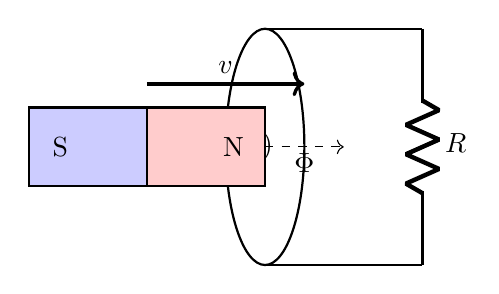
\begin{tikzpicture}
    % Coil
    \draw[thick] (0,0) ellipse (0.5 and 1.5);
    \draw[thick] (0,1.5) -- (2,1.5);
    \draw[thick] (0,-1.5) -- (2,-1.5);
    \draw[thick] (2,1.5) to[R, l=$R$] (2,-1.5);
    \node at (-1, 0) {Coil (N turns)};

    % Magnet
    \draw[thick, fill=blue!20] (-3, -0.5) rectangle (-1.5, 0.5);
    \node at (-2.6, 0) {S};
    \draw[thick, fill=red!20] (-1.5, -0.5) rectangle (0, 0.5);
    \node at (-0.4, 0) {N};
    
    % Motion arrow
    \draw[->, very thick] (-1.5, 0.8) -- (0.5, 0.8) node[midway, above] {$v$};
    
    % Flux lines
    \draw[dashed, ->] (0,0) -- (1,0);
    \node at (0.5, -0.2) {$\Phi$};
\end{tikzpicture}
\captionof{figure}{Faraday's Law Illustration}
\end{center}

\textbf{Applications:}
\begin{itemize}
    \item \keyword{Transformers}: Mutual induction principle
    \item \keyword{Generators}: Mechanical to electrical energy conversion
    \item \keyword{Inductors}: Self-induced EMF opposes current changes
\end{itemize}
\end{solutionbox}

\begin{mnemonicbox}
\mnemonic{"Flux Change Generates EMF" (dΦ/dt = EMF)}
\end{mnemonicbox}

\questionmarks{1(c)}{7}{Explain kirchhoff's voltage law and kirchhoff's current law with necessary diagram.}

\begin{solutionbox}
\textbf{Answer:}

\textbf{Kirchhoff's Laws Comparison:}
\begin{center}
\captionof{table}{Kirchhoff's Laws Comparison}
\begin{tabulary}{\linewidth}{|L|L|L|L|}
\hline
\textbf{Law} & \textbf{Statement} & \textbf{Mathematical Form} & \textbf{Application} \\ \hline
\textbf{KVL} & Sum of voltages in closed loop = 0 & $\Sigma V = 0$ & Series circuits \\ \hline
\textbf{KCL} & Sum of currents at node = 0 & $\Sigma I = 0$ & Parallel circuits \\ \hline
\end{tabulary}
\end{center}

\textbf{KVL Diagram:}
\begin{center}
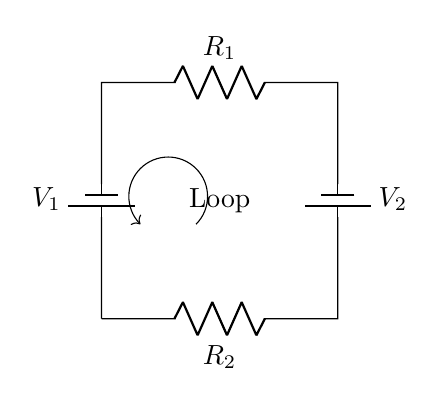
\begin{tikzpicture}
    \draw (0,0) to[battery1, l=$V_1$] (0,3)
    to[R, l=$R_1$] (3,3)
    to[battery1, l=$V_2$, invert] (3,0)
    to[R, l=$R_2$] (0,0);
    \node at (1.5, 1.5) {Loop};
    \draw[->] (1.2, 1.2) arc (-45:225:0.5);
\end{tikzpicture}
\captionof{figure}{KVL Closed Loop}
\end{center}

\textbf{KCL Diagram:}
\begin{center}
\begin{tikzpicture}
    \node[circle, fill, inner sep=2pt, label=above:Node] (N) at (0,0) {};
    \draw[<-] (N) -- (180:2) node[left] {$I_1$};
    \draw[<-] (N) -- (90:2) node[above] {$I_2$};
    \draw[->] (N) -- (0:2) node[right] {$I_3$};
    \draw[->] (N) -- (-90:2) node[below] {$I_4$};
\end{tikzpicture}
\captionof{figure}{KCL Node}
\end{center}

\textbf{Key Points:}
\begin{itemize}
    \item \keyword{KVL}: Algebraic sum considers voltage polarities
    \item \keyword{KCL}: Considers current directions (incoming vs outgoing)
    \item \keyword{Applications}: Circuit analysis, finding unknown values
\end{itemize}
\end{solutionbox}

\begin{mnemonicbox}
\mnemonic{"Voltage Loops, Current Nodes" (KVL for loops, KCL for nodes)}
\end{mnemonicbox}

\questionmarks{1(c OR)}{7}{Differentiate statically induced emf and dynamically induced emf}

\begin{solutionbox}
\textbf{Answer:}

\textbf{Static vs Dynamic EMF:}
\begin{center}
\captionof{table}{Static vs Dynamic EMF}
\begin{tabulary}{\linewidth}{|L|L|L|}
\hline
\textbf{Parameter} & \textbf{Statically Induced EMF} & \textbf{Dynamically Induced EMF} \\ \hline
\textbf{Cause} & Changing magnetic field & Relative motion between conductor and field \\ \hline
\textbf{Field} & Time-varying, conductor stationary & Steady field, conductor moving \\ \hline
\textbf{Examples} & Transformer, inductor & Generator, motor \\ \hline
\textbf{Formula} & $e = -N(d\Phi/dt)$ & $e = BLv$ \\ \hline
\textbf{Applications} & AC circuits, power supplies & Power generation, motors \\ \hline
\end{tabulary}
\end{center}

\textbf{Static EMF Types:}
\begin{itemize}
    \item \keyword{Self-induced}: Same coil creates and experiences flux change
    \item \keyword{Mutually induced}: One coil affects another coil
\end{itemize}

\textbf{Dynamic EMF Factors:}
\begin{itemize}
    \item \keyword{Magnetic field strength (B)}: Tesla
    \item \keyword{Conductor length (L)}: Meters
    \item \keyword{Velocity (v)}: m/s
\end{itemize}
\end{solutionbox}

\begin{mnemonicbox}
\mnemonic{"Static Stays, Dynamic Dances" (Static = stationary, Dynamic = motion)}
\end{mnemonicbox}

\questionmarks{2(a)}{3}{Explain various types of losses in transformer.}

\begin{solutionbox}
\textbf{Answer:}

\textbf{Transformer Losses:}
\begin{center}
\captionof{table}{Transformer Losses}
\begin{tabulary}{\linewidth}{|L|L|L|L|}
\hline
\textbf{Loss Type} & \textbf{Cause} & \textbf{Location} & \textbf{Characteristics} \\ \hline
\textbf{Iron Loss} & Hysteresis + Eddy currents & Core & Constant, frequency dependent \\ \hline
\textbf{Copper Loss} & $I^2R$ heating & Windings & Variable with load \\ \hline
\textbf{Stray Loss} & Leakage flux & Overall & Minimal \\ \hline
\end{tabulary}
\end{center}

\textbf{Iron Losses:}
\begin{itemize}
    \item \keyword{Hysteresis loss}: Magnetic domain reversal energy
    \item \keyword{Eddy current loss}: Circulating currents in core
\end{itemize}

\textbf{Copper Losses:}
\begin{itemize}
    \item \keyword{Primary winding}: $I_1^2R_1$
    \item \keyword{Secondary winding}: $I_2^2R_2$
\end{itemize}
\end{solutionbox}

\begin{mnemonicbox}
\mnemonic{"Iron Core, Copper Coil" (Location of main losses)}
\end{mnemonicbox}

\questionmarks{2(b)}{4}{Explain working principle of transformer.}

\begin{solutionbox}
\textbf{Answer:}

\textbf{Working Principle:}
\keyword{Mutual electromagnetic induction} between primary and secondary windings through common magnetic core.

\textbf{Diagram:}
\begin{center}
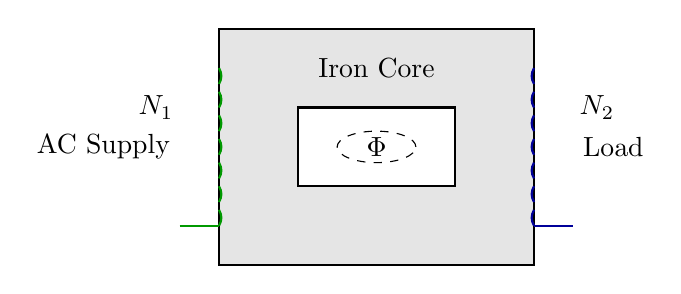
\begin{tikzpicture}
    % Core
    \draw[thick, fill=gray!20] (0,0) rectangle (4,3);
    \draw[thick, fill=white] (1,1) rectangle (3,2);
    \node at (2, 2.5) {Iron Core};
    
    % Primary
    \draw[green!60!black, thick] (-0.5, 0.5) -- (0, 0.5);
    \foreach \y in {0.5, 0.8, ..., 2.5}
        \draw[green!60!black, thick] (0, \y) to[bend right] (0, \y+0.2);
    \node[left] at (-0.5, 1.5) {AC Supply};
    \node at (-0.8, 2) {$N_1$};
    
    % Secondary
    \draw[blue!60!black, thick] (4, 0.5) -- (4.5, 0.5);
    \foreach \y in {0.5, 0.8, ..., 2.5}
        \draw[blue!60!black, thick] (4, \y) to[bend left] (4, \y+0.2);
    \node[right] at (4.5, 1.5) {Load};
    \node at (4.8, 2) {$N_2$};
    
    % Flux
    \draw[dashed, ->] (2, 1.5) ellipse (0.5 and 0.2);
    \node at (2, 1.5) {$\Phi$};
\end{tikzpicture}
\captionof{figure}{Transformer Principle}
\end{center}

\textbf{Operation Steps:}
\begin{itemize}
    \item \textbf{Step 1}: AC current in primary creates alternating flux
    \item \textbf{Step 2}: Flux links secondary through core
    \item \textbf{Step 3}: Changing flux induces EMF in secondary
    \item \textbf{Step 4}: Secondary EMF drives current through load
\end{itemize}

\textbf{Key Relations:}
\begin{itemize}
    \item \keyword{Voltage ratio}: $V_2/V_1 = N_2/N_1$
    \item \keyword{Current ratio}: $I_1/I_2 = N_2/N_1$
\end{itemize}
\end{solutionbox}

\begin{mnemonicbox}
\mnemonic{"Primary Produces, Secondary Supplies" (Energy transfer direction)}
\end{mnemonicbox}

\questionmarks{2(c)}{7}{Derive emf equation of transformer.}

\begin{solutionbox}
\textbf{Answer:}

\textbf{Given Parameters:}
\begin{itemize}
    \item $N_1$: Primary turns, $N_2$: Secondary turns
    \item $\Phi_m$: Maximum flux, $f$: Frequency
\end{itemize}

\textbf{EMF Derivation:}

\textbf{Step 1: Flux Variation}
\[ \Phi = \Phi_m \sin(2\pi ft) \]

\textbf{Step 2: Rate of Flux Change}
\[ \frac{d\Phi}{dt} = 2\pi f \Phi_m \cos(2\pi ft) \]

\textbf{Step 3: Maximum Rate}
\[ \left(\frac{d\Phi}{dt}\right)_{max} = 2\pi f \Phi_m \]

\textbf{Step 4: RMS EMF Formula}
\begin{align*}
E_1 &= 4.44 \times f \times N_1 \times \Phi_m \\
E_2 &= 4.44 \times f \times N_2 \times \Phi_m
\end{align*}

\textbf{EMF Equation Components:}
\begin{center}
\captionof{table}{EMF Equation Components}
\begin{tabulary}{\linewidth}{|L|L|L|}
\hline
\textbf{Symbol} & \textbf{Parameter} & \textbf{Units} \\ \hline
$E$ & RMS EMF & Volts \\ \hline
$f$ & Frequency & Hz \\ \hline
$N$ & Number of turns & - \\ \hline
$\Phi_m$ & Maximum flux & Weber \\ \hline
$4.44$ & Form factor constant & - \\ \hline
\end{tabulary}
\end{center}

\textbf{Transformation Ratio:}
\[ K = \frac{E_2}{E_1} = \frac{N_2}{N_1} \]
\end{solutionbox}

\begin{mnemonicbox}
\mnemonic{"Four-Forty-Four Flux Formula" (4.44 factor)}
\end{mnemonicbox}

\questionmarks{2(a OR)}{3}{Write application of transformer.}

\begin{solutionbox}
\textbf{Answer:}

\textbf{Transformer Applications:}
\begin{center}
\captionof{table}{Transformer Applications}
\begin{tabulary}{\linewidth}{|L|L|L|}
\hline
\textbf{Application} & \textbf{Purpose} & \textbf{Voltage Level} \\ \hline
\textbf{Power transmission} & Reduce transmission losses & Step-up (400kV) \\ \hline
\textbf{Distribution} & Safe voltage for consumers & Step-down (230V) \\ \hline
\textbf{Isolation} & Electrical isolation & 1:1 ratio \\ \hline
\textbf{Electronic circuits} & DC power supplies & Step-down \\ \hline
\end{tabulary}
\end{center}

\textbf{Industrial Applications:}
\begin{itemize}
    \item \keyword{Welding transformers}: High current, low voltage
    \item \keyword{Instrument transformers}: Measurement and protection
    \item \keyword{Audio transformers}: Impedance matching
\end{itemize}
\end{solutionbox}

\begin{mnemonicbox}
\mnemonic{"Power Distribution Isolation Electronics" (Main application areas)}
\end{mnemonicbox}

\questionmarks{2(b OR)}{4}{Write equation for back emf and torque of D.C motor.}

\begin{solutionbox}
\textbf{Answer:}

\textbf{Back EMF Equation:}
\[ E_b = \frac{\phi Z N P}{60 A} \]

\textbf{Simplified Form:}
\[ E_b = K \phi N \]

\textbf{Torque Equation:}
\[ T = \frac{\phi Z I_a P}{2\pi A} \]

\textbf{Simplified Form:}
\[ T = K \phi I_a \]

\textbf{Symbol Definitions:}
\begin{center}
\captionof{table}{Symbol Definitions}
\begin{tabulary}{\linewidth}{|L|L|L|}
\hline
\textbf{Symbol} & \textbf{Parameter} & \textbf{Units} \\ \hline
$E_b$ & Back EMF & Volts \\ \hline
$T$ & Torque & N-m \\ \hline
$\phi$ & Flux per pole & Weber \\ \hline
$N$ & Speed & RPM \\ \hline
$I_a$ & Armature current & Amperes \\ \hline
$K$ & Motor constant & - \\ \hline
\end{tabulary}
\end{center}
\end{solutionbox}

\begin{mnemonicbox}
\mnemonic{"Back EMF opposes, Torque proposes" (EMF opposes supply, torque drives rotation)}
\end{mnemonicbox}

\questionmarks{2(c OR)}{7}{Explain construction and working of D.C. motor with necessary figure}

\begin{solutionbox}
\textbf{Answer:}

\textbf{Construction Components:}
\begin{center}
\captionof{table}{DC Motor Parts}
\begin{tabulary}{\linewidth}{|L|L|L|}
\hline
\textbf{Component} & \textbf{Function} & \textbf{Material} \\ \hline
\textbf{Stator} & Provides magnetic field & Cast iron/steel \\ \hline
\textbf{Rotor/Armature} & Rotating part & Silicon steel laminations \\ \hline
\textbf{Commutator} & Current direction reversal & Copper segments \\ \hline
\textbf{Brushes} & Current collection & Carbon \\ \hline
\textbf{Field windings} & Electromagnets & Copper wire \\ \hline
\end{tabulary}
\end{center}

\textbf{Construction Diagram:}
\begin{center}
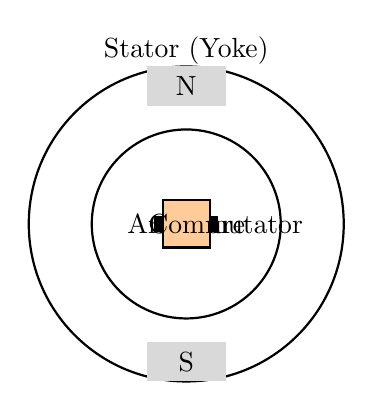
\begin{tikzpicture}
    % Stator
    \draw[thick] (0,0) circle (2);
    \node at (0, 2.2) {Stator (Yoke)};
    
    % Poles
    \fill[gray!30] (-0.5, 1.5) rectangle (0.5, 2); % N Pole Top
    \node at (0, 1.75) {N};
    \fill[gray!30] (-0.5, -2) rectangle (0.5, -1.5); % S Pole Bottom
    \node at (0, -1.75) {S};
    
    % Armature
    \draw[thick, fill=white] (0,0) circle (1.2);
    \node at (0,0) {Armature};
    
    % Commutator/Brushes
    \draw[thick, fill=orange!40] (-0.3, -0.3) rectangle (0.3, 0.3);
    \node at (0.5, 0) {Commutator};
    \draw[fill=black] (-0.4, -0.1) rectangle (-0.3, 0.1); % Brush
    \draw[fill=black] (0.3, -0.1) rectangle (0.4, 0.1); % Brush
\end{tikzpicture}
\captionof{figure}{DC Motor Construction}
\end{center}

\textbf{Working Principle:}
\begin{itemize}
    \item \textbf{Step 1}: Current flows through armature conductors
    \item \textbf{Step 2}: Magnetic field interacts with current
    \item \textbf{Step 3}: Force generated by Fleming's left-hand rule
    \item \textbf{Step 4}: Commutator reverses current direction
    \item \textbf{Step 5}: Continuous rotation maintained
\end{itemize}

\textbf{Force Equation:}
\[ F = B \times I \times L \]
\end{solutionbox}

\begin{mnemonicbox}
\mnemonic{"Current Creates Circular motion" (Current interaction produces rotation)}
\end{mnemonicbox}

\questionmarks{3(a)}{3}{Explain construction of transformer.}

\begin{solutionbox}
\textbf{Answer:}

\textbf{Transformer Construction:}
\begin{center}
\captionof{table}{Transformer Construction}
\begin{tabulary}{\linewidth}{|L|L|L|}
\hline
\textbf{Component} & \textbf{Material} & \textbf{Function} \\ \hline
\textbf{Core} & Silicon steel laminations & Magnetic flux path \\ \hline
\textbf{Primary winding} & Copper/Aluminum & Input energy \\ \hline
\textbf{Secondary winding} & Copper/Aluminum & Output energy \\ \hline
\textbf{Insulation} & Varnish/Paper & Electrical isolation \\ \hline
\textbf{Tank} & Steel & Oil containment \& cooling \\ \hline
\end{tabulary}
\end{center}

\textbf{Core Types:}
\begin{itemize}
    \item \keyword{Shell type}: Windings surrounded by core
    \item \keyword{Core type}: Core surrounded by windings
\end{itemize}

\textbf{Cooling Methods:}
\begin{itemize}
    \item \keyword{Air cooling}: Small transformers
    \item \keyword{Oil cooling}: Large transformers with radiators
\end{itemize}
\end{solutionbox}

\begin{mnemonicbox}
\mnemonic{"Core Carries Current Carefully" (Core design importance)}
\end{mnemonicbox}

\questionmarks{3(b)}{4}{Explain application of DC motor}

\begin{solutionbox}
\textbf{Answer:}

\textbf{DC Motor Applications:}
\begin{center}
\captionof{table}{DC Motor Applications}
\begin{tabulary}{\linewidth}{|L|L|L|}
\hline
\textbf{Motor Type} & \textbf{Speed Characteristic} & \textbf{Applications} \\ \hline
\textbf{Shunt} & Constant speed & Fans, pumps, lathes \\ \hline
\textbf{Series} & Variable speed & Traction, cranes \\ \hline
\textbf{Compound} & Moderate variation & Elevators, compressors \\ \hline
\end{tabulary}
\end{center}

\textbf{Industrial Applications:}
\begin{itemize}
    \item \keyword{Shunt motors}: Machine tools requiring constant speed
    \item \keyword{Series motors}: Electric vehicles, starting heavy loads
    \item \keyword{Compound motors}: Rolling mills, punch presses
\end{itemize}

\textbf{Advantages:}
\begin{itemize}
    \item \keyword{Easy speed control}: Voltage/field control
    \item \keyword{High starting torque}: Series motors
    \item \keyword{Reversible operation}: Change field/armature polarity
\end{itemize}
\end{solutionbox}

\begin{mnemonicbox}
\mnemonic{"Shunt Stays, Series Speeds" (Speed characteristics)}
\end{mnemonicbox}

\questionmarks{3(c)}{7}{Explain different types of DC motor.}

\begin{solutionbox}
\textbf{Answer:}

\textbf{DC Motor Classification:}
\begin{center}
\captionof{table}{DC Motor Classification}
\begin{tabulary}{\linewidth}{|L|L|L|L|}
\hline
\textbf{Type} & \textbf{Field Connection} & \textbf{Speed-Torque} & \textbf{Applications} \\ \hline
\textbf{Shunt} & Parallel to armature & Constant speed, low starting torque & Fans, pumps \\ \hline
\textbf{Series} & Series with armature & Variable speed, high starting torque & Traction \\ \hline
\textbf{Compound} & Both series \& shunt & Moderate characteristics & General purpose \\ \hline
\end{tabulary}
\end{center}

\textbf{Shunt Motor Diagram:}
\begin{center}
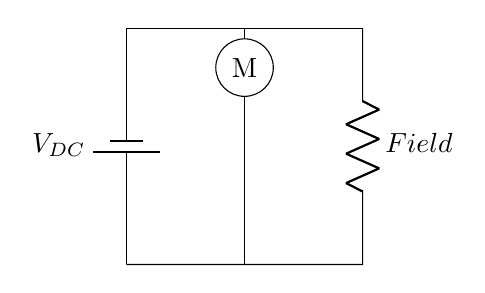
\begin{tikzpicture}
    \draw (0,0) to[battery1, l=$V_{DC}$] (0,3) -- (3,3);
    \draw (3,3) to[R, l=$Field$] (3,0) -- (0,0);
    \draw (1.5,3) to[short] (1.5,2.5) node[circle, draw, fill=white] {M} -- (1.5,0);
\end{tikzpicture}
\captionof{figure}{DC Shunt Motor}
\end{center}

\textbf{Characteristics:}
\begin{itemize}
    \item \textbf{Shunt}: Speed $\propto (V - I_aR_a)/\phi$
    \item \textbf{Series}: High starting torque, speed varies with load
    \item \textbf{Compound}: Combines advantages of both types
\end{itemize}

\textbf{Speed Control Methods:}
\begin{itemize}
    \item \keyword{Armature control}: Vary armature voltage
    \item \keyword{Field control}: Vary field current
    \item \keyword{Resistance control}: Add external resistance
\end{itemize}
\end{solutionbox}

\begin{mnemonicbox}
\mnemonic{"Shunt Steady, Series Strong, Compound Combined" (Key characteristics)}
\end{mnemonicbox}

\questionmarks{3(a OR)}{3}{Explain transformation ratio of transformer.}

\begin{solutionbox}
\textbf{Answer:}

\textbf{Definition:}
Transformation ratio ($K$) is the ratio of secondary to primary voltage or turns.

\textbf{Mathematical Expression:}
\[ K = \frac{N_2}{N_1} = \frac{E_2}{E_1} = \frac{V_2}{V_1} \]

\textbf{Transformation Ratio Types:}
\begin{center}
\captionof{table}{Transformation Ratio Types}
\begin{tabulary}{\linewidth}{|L|L|L|L|}
\hline
\textbf{Ratio} & \textbf{Type} & \textbf{Voltage Change} & \textbf{Applications} \\ \hline
$K > 1$ & Step-up & Increases & Power transmission \\ \hline
$K < 1$ & Step-down & Decreases & Distribution \\ \hline
$K = 1$ & Isolation & Same & Safety isolation \\ \hline
\end{tabulary}
\end{center}

\textbf{Current Relationship:}
\[ \frac{I_1}{I_2} = \frac{N_2}{N_1} = K \]

\textbf{Power Relationship:}
\[ P_1 = P_2 \text{ (Ideal transformer)} \]
\end{solutionbox}

\begin{mnemonicbox}
\mnemonic{"Turns Tell Transformation" (Turns ratio determines voltage ratio)}
\end{mnemonicbox}

\questionmarks{3(b OR)}{4}{Write application of autotransformer.}

\begin{solutionbox}
\textbf{Answer:}

\textbf{Autotransformer Applications:}
\begin{center}
\captionof{table}{Autotransformer Applications}
\begin{tabulary}{\linewidth}{|L|L|L|}
\hline
\textbf{Application} & \textbf{Advantage} & \textbf{Voltage Range} \\ \hline
\textbf{Motor starting} & Reduced starting current & 50-80\% of rated \\ \hline
\textbf{Voltage regulation} & Fine voltage adjustment & $\pm$10\% variation \\ \hline
\textbf{Laboratory} & Variable voltage source & 0-110\% of input \\ \hline
\textbf{Power systems} & Economic transmission & Close voltage ratios \\ \hline
\end{tabulary}
\end{center}

\textbf{Advantages:}
\begin{itemize}
    \item \keyword{Economy}: Less copper and iron required
    \item \keyword{Efficiency}: Higher than two-winding transformer
    \item \keyword{Size}: Compact design
    \item \keyword{Regulation}: Better voltage regulation
\end{itemize}

\textbf{Limitations:}
\begin{itemize}
    \item \keyword{No isolation}: Common electrical connection
    \item \keyword{Safety}: Higher fault current
\end{itemize}
\end{solutionbox}

\begin{mnemonicbox}
\mnemonic{"Auto Adjusts Advantageously" (Automatic voltage adjustment benefit)}
\end{mnemonicbox}

\questionmarks{3(c OR)}{7}{Explain speed control of DC shunt motor}

\begin{solutionbox}
\textbf{Answer:}

\textbf{Speed Control Methods:}
\begin{center}
\captionof{table}{Speed Control Methods}
\begin{tabulary}{\linewidth}{|L|L|L|L|}
\hline
\textbf{Method} & \textbf{Range} & \textbf{Efficiency} & \textbf{Applications} \\ \hline
\textbf{Armature control} & Below rated speed & High & Precise speed control \\ \hline
\textbf{Field control} & Above rated speed & High & Constant power drives \\ \hline
\textbf{Resistance control} & Below rated speed & Low & Simple applications \\ \hline
\end{tabulary}
\end{center}

\textbf{Armature Control Diagram:}
\begin{center}
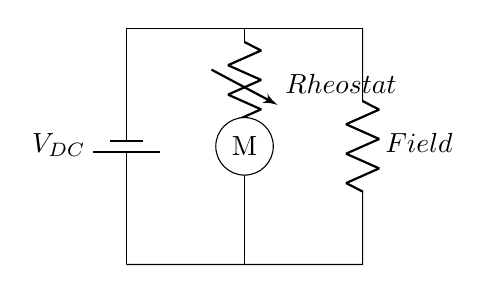
\begin{tikzpicture}
    \draw (0,0) to[battery1, l=$V_{DC}$] (0,3) -- (3,3);
    \draw (3,3) to[R, l=$Field$] (3,0) -- (0,0);
    \draw (1.5,3) to[vR, l=$Rheostat$] (1.5,1.5) node[circle, draw, fill=white] {M} -- (1.5,0);
\end{tikzpicture}
\captionof{figure}{Armature Control Method}
\end{center}

\textbf{Speed Equations:}
\begin{itemize}
    \item \keyword{Armature control}: $N \propto (V - I_aR_a)/\phi$
    \item \keyword{Field control}: $N \propto V/\phi$
    \item \keyword{Resistance control}: $N \propto (V - I_a(R_a + R_{ext}))/\phi$
\end{itemize}

\textbf{Modern Methods:}
\begin{itemize}
    \item \keyword{Chopper control}: PWM voltage control
    \item \keyword{Ward-Leonard system}: Motor-generator set
    \item \keyword{Electronic control}: Thyristor/IGBT drives
\end{itemize}

\textbf{Characteristics:}
\begin{itemize}
    \item \keyword{Smooth control}: Stepless speed variation
    \item \keyword{Efficiency}: Armature control most efficient
    \item \keyword{Cost}: Field control economical
\end{itemize}
\end{solutionbox}

\begin{mnemonicbox}
\mnemonic{"Armature Accurate, Field Fast, Resistance Rough" (Control characteristics)}
\end{mnemonicbox}

\questionmarks{4(a)}{3}{Explain vector representation of alternating EMF.}

\begin{solutionbox}
\textbf{Answer:}

\textbf{Vector Representation:}
Alternating EMF can be represented as a rotating vector (phasor) with constant magnitude and angular velocity.

\textbf{Mathematical Form:}
\[ e = E_m \sin(\omega t + \phi) \]

\textbf{Diagram:}
\begin{center}
\begin{tikzpicture}
    % Axes
    \draw[->] (-0.5,0) -- (3,0) node[right] {Reference};
    \draw[->] (0,-0.5) -- (0,3);
    
    % Phasor
    \draw[thick, ->] (0,0) -- (45:2.5) node[right] {$E_m$};
    \draw (0.5,0) arc (0:45:0.5) node[midway, right] {$\phi$};
    
    % Projection
    %\draw[dashed] (45:2.5) -- (1.76, 0);
    
    % Angular velocity
    \draw[->] (0.8, 0.8) arc (45:135:0.5) node[midway, above] {$\omega$};
\end{tikzpicture}
\captionof{figure}{EMF Phasor Diagram}
\end{center}

\textbf{Vector Parameters:}
\begin{center}
\captionof{table}{Vector Parameters}
\begin{tabulary}{\linewidth}{|L|L|L|L|}
\hline
\textbf{Parameter} & \textbf{Symbol} & \textbf{Units} & \textbf{Description} \\ \hline
\textbf{Magnitude} & $E_m$ & Volts & Maximum EMF \\ \hline
\textbf{Angular velocity} & $\omega$ & rad/s & Rotation speed \\ \hline
\textbf{Phase angle} & $\phi$ & Degrees & Initial phase \\ \hline
\textbf{Frequency} & $f = \omega/2\pi$ & Hz & Cycles per second \\ \hline
\end{tabulary}
\end{center}

\textbf{Advantages:}
\begin{itemize}
    \item \keyword{Visual representation}: Easy to understand phase relationships
    \item \keyword{Mathematical simplification}: Complex calculations made easier
\end{itemize}
\end{solutionbox}

\begin{mnemonicbox}
\mnemonic{"Vectors Visualize Voltage Variation" (Phasor representation benefits)}
\end{mnemonicbox}

\questionmarks{4(b)}{4}{Define following terms w.r.t Alternating current: RMS value, Average value, Frequency, Time period}

\begin{solutionbox}
\textbf{Answer:}

\textbf{AC Parameters Definition:}
\begin{center}
\captionof{table}{AC Parameters Definition}
\begin{tabulary}{\linewidth}{|L|L|L|L|}
\hline
\textbf{Term} & \textbf{Definition} & \textbf{Formula} & \textbf{Units} \\ \hline
\textbf{RMS Value} & Effective value producing same heating & $I_m/\sqrt{2}$ & Amperes \\ \hline
\textbf{Average Value} & Mean value over half cycle & $2I_m/\pi$ & Amperes \\ \hline
\textbf{Frequency} & Number of cycles per second & $f = 1/T$ & Hz \\ \hline
\textbf{Time Period} & Time for one complete cycle & $T = 1/f$ & Seconds \\ \hline
\end{tabulary}
\end{center}

\textbf{Mathematical Relations:}
\begin{itemize}
    \item \keyword{Form Factor}: RMS/Average = $\pi/2\sqrt{2} = 1.11$
    \item \keyword{Peak Factor}: Peak/RMS = $\sqrt{2} = 1.414$
    \item \keyword{Angular frequency}: $\omega = 2\pi f$
\end{itemize}
\end{solutionbox}

\begin{mnemonicbox}
\mnemonic{"Really Mean Square, Average Frequency Time" (Key AC parameters)}
\end{mnemonicbox}

\questionmarks{4(c)}{7}{Derive equation for relation between line and phase voltage and current in star connection}

\begin{solutionbox}
\textbf{Answer:}

\textbf{Star Connection Diagram:}
\begin{center}
\begin{tikzpicture}
    % Star Point
    \coordinate (N) at (0,0);
    \node[below left] at (N) {N};
    
    % Phases
    \draw (N) -- (90:2) node[above] {R} coordinate (R);
    \draw (N) -- (210:2) node[below left] {Y} coordinate (Y);
    \draw (N) -- (330:2) node[below right] {B} coordinate (B);
    
    % Lines
    \draw[->] (R) -- ++(0,0.5) node[above] {Line R};
    \draw[->] (Y) -- ++(-0.4,-0.2) node[left] {Line Y};
    \draw[->] (B) -- ++(0.4,-0.2) node[right] {Line B};
    
    % Voltages
    \node at (0.2, 1) {$V_{ph}$};
\end{tikzpicture}
\captionof{figure}{Star Connection}
\end{center}

\textbf{Voltage Relations:}
\begin{itemize}
    \item \keyword{Phase Voltages}: $V_R, V_Y, V_B$ (with respect to neutral)
    \item \keyword{Line Voltages}: $V_{RY}, V_{YB}, V_{BR}$ (between lines)
\end{itemize}

\textbf{Phasor Analysis:}
\[ V_{RY} = V_R - V_Y \]

\textbf{For balanced system:}
\begin{itemize}
    \item Phase voltages are equal in magnitude: $V_R = V_Y = V_B = V_{ph}$
    \item Phase difference = 120$^\circ$
\end{itemize}

\textbf{Vector Addition:}
Using phasor diagram and cosine rule:
\begin{align*}
V_L &= \sqrt{V_{ph}^2 + V_{ph}^2 - 2V_{ph}V_{ph}\cos(120^\circ)} \\
V_L &= \sqrt{2V_{ph}^2 + V_{ph}^2} = \sqrt{3} \times V_{ph}
\end{align*}

\textbf{Final Relations:}

\textbf{Star Connection Relations:}
\begin{center}
\captionof{table}{Star Connection Relations}
\begin{tabulary}{\linewidth}{|L|L|}
\hline
\textbf{Parameter} & \textbf{Relationship} \\ \hline
\textbf{Line Voltage} & $V_L = \sqrt{3} \times V_{ph}$ \\ \hline
\textbf{Line Current} & $I_L = I_{ph}$ \\ \hline
\textbf{Power} & $P = \sqrt{3} V_L I_L \cos\phi$ \\ \hline
\end{tabulary}
\end{center}
\end{solutionbox}

\begin{mnemonicbox}
\mnemonic{"Star Scales Voltage, Same current" ($\sqrt{3}$ factor for voltage, current unchanged)}
\end{mnemonicbox}

\questionmarks{4(a OR)}{3}{Explain vector representation of alternating current.}

\begin{solutionbox}
\textbf{Answer:}

\textbf{Vector Representation:}
AC current represented as rotating phasor with magnitude and phase angle.

\textbf{Mathematical Expression:}
\[ i = I_m \sin(\omega t + \phi) \]

\textbf{Phasor Diagram:}
\begin{center}
\begin{tikzpicture}
    % Axes
    \draw[->] (-0.5,0) -- (3,0) node[right] {Reference};
    \draw[->] (0,-0.5) -- (0,3);
    
    % Phasor
    \draw[thick, ->] (0,0) -- (60:2.5) node[right] {$I_m$};
    \draw (0.5,0) arc (0:60:0.5) node[midway, right] {$\phi$};
    
    % Angular velocity
    \draw[->] (0.8, 0.8) arc (45:135:0.5) node[midway, above] {$\omega t$};
\end{tikzpicture}
\captionof{figure}{Current Phasor Diagram}
\end{center}

\textbf{Current Vector Elements:}
\begin{center}
\captionof{table}{Current Vector Elements}
\begin{tabulary}{\linewidth}{|L|L|L|}
\hline
\textbf{Element} & \textbf{Symbol} & \textbf{Description} \\ \hline
\textbf{Magnitude} & $I_m$ & Peak current value \\ \hline
\textbf{Phase} & $\phi$ & Leading/lagging angle \\ \hline
\textbf{Angular velocity} & $\omega$ & Rotation speed \\ \hline
\textbf{RMS value} & $I = I_m/\sqrt{2}$ & Effective current \\ \hline
\end{tabulary}
\end{center}
\end{solutionbox}

\begin{mnemonicbox}
\mnemonic{"Current Circles Continuously" (Rotating phasor concept)}
\end{mnemonicbox}

\questionmarks{4(b OR)}{4}{Define following terms w.r.t Alternating current: Form factor, Peak factor, Angular velocity, Amplitude}

\begin{solutionbox}
\textbf{Answer:}

\textbf{AC Current Parameters:}
\begin{center}
\captionof{table}{AC Current Parameters}
\begin{tabulary}{\linewidth}{|L|L|L|L|}
\hline
\textbf{Term} & \textbf{Definition} & \textbf{Formula} & \textbf{Typical Value} \\ \hline
\textbf{Form Factor} & RMS/Average value ratio & $I_{rms}/I_{avg}$ & 1.11 (sine wave) \\ \hline
\textbf{Peak Factor} & Peak/RMS value ratio & $I_m/I_{rms}$ & 1.414 (sine wave) \\ \hline
\textbf{Angular Velocity} & Rate of phase change & $\omega = 2\pi f$ & 314 rad/s (50Hz) \\ \hline
\textbf{Amplitude} & Maximum instantaneous value & $I_m$ & Peak current \\ \hline
\end{tabulary}
\end{center}

\textbf{Practical Significance:}
\begin{itemize}
    \item \keyword{Design considerations}: Peak factors for insulation
    \item \keyword{Waveform analysis}: Form factors for distortion
    \item \keyword{Synchronization}: Angular velocity for timing
\end{itemize}
\end{solutionbox}

\begin{mnemonicbox}
\mnemonic{"Form Peak Angular Amplitude" (Four key factors)}
\end{mnemonicbox}

\questionmarks{4(c OR)}{7}{Derive equation for relation between line and phase voltage and current in delta connection}

\begin{solutionbox}
\textbf{Answer:}

\textbf{Delta Connection Diagram:}
\begin{center}
\begin{tikzpicture}
    % Delta
    \draw (0,0) coordinate (C) -- (3,0) coordinate (B) -- (1.5, 2.6) coordinate (A) -- cycle;
    \node[above] at (A) {A};
    \node[right] at (B) {B};
    \node[left] at (C) {C};
    
    % Lines
    \draw[->] (A) -- ++(0,1) node[above] {$I_A$};
    \draw[->] (B) -- ++(1,-0.5) node[right] {$I_B$};
    \draw[->] (C) -- ++(-1,-0.5) node[left] {$I_C$};
    
    % Currents inside
    \draw[->] (1.8, 2) -- (2.5, 0.8) node[midway, right] {$I_{AB}$};
\end{tikzpicture}
\captionof{figure}{Delta Connection}
\end{center}

\textbf{Voltage Relations:}
In delta connection, line voltage equals phase voltage:
\[ V_L = V_{ph} \]

\textbf{Current Analysis:}
Each line current is vector sum of two phase currents.

\textbf{For Line Current $I_A$:}
\[ I_A = I_{AB} - I_{CA} \]

\textbf{Phasor Analysis:}
For balanced system with phase currents equal in magnitude:
\begin{itemize}
    \item $I_{AB} = I_{CA} = I_{CB} = I_{ph}$
    \item Phase difference between currents = 120$^\circ$
\end{itemize}

\textbf{Vector Subtraction:}
\[ I_A = I_{AB} - I_{CA} = I_{AB} - (-I_{CA}) \]

Using phasor diagram:
\begin{align*}
I_L &= \sqrt{I_{ph}^2 + I_{ph}^2 - 2I_{ph}I_{ph}\cos(60^\circ)} \\
I_L &= \sqrt{2I_{ph}^2 - I_{ph}^2} = \sqrt{3} \times I_{ph}
\end{align*}

\textbf{Delta Connection Relations:}
\begin{center}
\captionof{table}{Delta Connection Relations}
\begin{tabulary}{\linewidth}{|L|L|}
\hline
\textbf{Parameter} & \textbf{Relationship} \\ \hline
\textbf{Line Voltage} & $V_L = V_{ph}$ \\ \hline
\textbf{Line Current} & $I_L = \sqrt{3} \times I_{ph}$ \\ \hline
\textbf{Power} & $P = \sqrt{3} V_L I_L \cos\phi$ \\ \hline
\end{tabulary}
\end{center}
\end{solutionbox}

\begin{mnemonicbox}
\mnemonic{"Delta Doubles current, Same voltage" ($\sqrt{3}$ factor for current, voltage unchanged)}
\end{mnemonicbox}

\questionmarks{5(a)}{3}{Explain AC through pure resistor with necessary circuit and waveform.}

\begin{solutionbox}
\textbf{Answer:}

\textbf{Circuit Diagram:}
\begin{center}
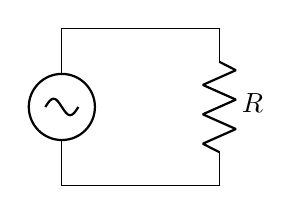
\begin{tikzpicture}
    \draw (0,0) to[sinusoidal voltage source] (0,2) -- (2,2)
    to[R, l=$R$] (2,0) -- (0,0);
\end{tikzpicture}
\captionof{figure}{AC through Resistor}
\end{center}

\textbf{Waveform:}
\begin{center}
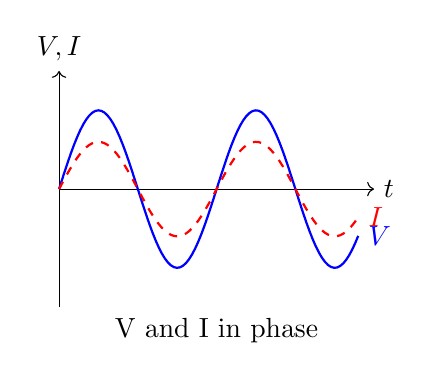
\begin{tikzpicture}
    \draw[->] (0,0) -- (4,0) node[right] {$t$};
    \draw[->] (0,-1.5) -- (0,1.5) node[above] {$V, I$};
    \draw[blue, thick] plot[domain=0:3.8, samples=100] (\x, {sin(3.14*\x r)}) node[right] {$V$};
    \draw[red, dashed, thick] plot[domain=0:3.8, samples=100] (\x, {0.6*sin(3.14*\x r)}) node[right] {$I$};
    \node at (2, -1.8) {V and I in phase};
\end{tikzpicture}
\captionof{figure}{Resistive Waveforms}
\end{center}

\textbf{AC through Resistor:}
\begin{center}
\captionof{table}{AC through Resistor}
\begin{tabulary}{\linewidth}{|L|L|L|}
\hline
\textbf{Parameter} & \textbf{Relationship} & \textbf{Phase} \\ \hline
\textbf{Ohm's Law} & $V = IR$ & Same phase \\ \hline
\textbf{Power} & $P = VI = I^2R$ & Always positive \\ \hline
\textbf{Impedance} & $Z = R$ & Purely resistive \\ \hline
\end{tabulary}
\end{center}
\end{solutionbox}

\begin{mnemonicbox}
\mnemonic{"Resistor Refuses phase Shift" (No phase difference)}
\end{mnemonicbox}

\questionmarks{5(b)}{4}{Define following terms w.r.t Alternating current: Impedance, Phase angle, Power factor, Reactive power}

\begin{solutionbox}
\textbf{Answer:}

\textbf{AC Circuit Parameters:}
\begin{center}
\captionof{table}{AC Circuit Parameters}
\begin{tabulary}{\linewidth}{|L|L|L|L|}
\hline
\textbf{Term} & \textbf{Definition} & \textbf{Formula} & \textbf{Units} \\ \hline
\textbf{Impedance} & Total opposition to AC current & $Z = \sqrt{R^2 + X^2}$ & Ohms \\ \hline
\textbf{Phase Angle} & Angle between V and I & $\phi = \tan^{-1}(X/R)$ & Degrees \\ \hline
\textbf{Power Factor} & Cosine of phase angle & $PF = \cos\phi = R/Z$ & - \\ \hline
\textbf{Reactive Power} & Power in reactive components & $Q = VI \sin\phi$ & VAR \\ \hline
\end{tabulary}
\end{center}

\textbf{Power Triangle:}
\[ S^2 = P^2 + Q^2 \]
\end{solutionbox}

\begin{mnemonicbox}
\mnemonic{"Impedance Phase Power Quadrature" (Four key AC parameters)}
\end{mnemonicbox}

\questionmarks{5(c)}{7}{Enlist different protective device and explain construction and working of any one protective device.}

\begin{solutionbox}
\textbf{Answer:}

\textbf{Protective Devices:}
\begin{center}
\captionof{table}{Protective Devices}
\begin{tabulary}{\linewidth}{|L|L|L|}
\hline
\textbf{Device} & \textbf{Protection Against} & \textbf{Application} \\ \hline
\textbf{Fuse} & Overcurrent & Low/Medium voltage \\ \hline
\textbf{MCB} & Overload, Short circuit & Domestic/Commercial \\ \hline
\textbf{ELCB} & Earth leakage & Safety protection \\ \hline
\textbf{Relay} & Various faults & Industrial systems \\ \hline
\textbf{Surge arrester} & Overvoltage & Transmission lines \\ \hline
\end{tabulary}
\end{center}

\textbf{MCB (Miniature Circuit Breaker) - Detailed Explanation:}

\textbf{Construction:}
\begin{center}
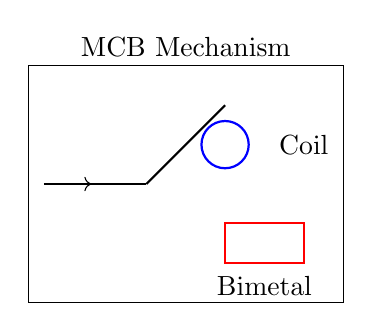
\begin{tikzpicture}
    % Box
    \draw (0,0) rectangle (4,3);
    \node[above] at (2,3) {MCB Mechanism};
    
    % Mechanism
    \draw[thick] (0.5, 1.5) -- (1.5, 1.5); % Contact
    \draw[thick] (1.5, 1.5) -- (2.5, 2.5); % Moving arm
    \draw[thick, red] (2.5, 1.0) rectangle (3.5, 0.5); % Bimetal
    \node at (3, 0.2) {Bimetal};
    \draw[thick, blue] (2.5, 2.0) circle (0.3); % Coil
    \node at (3.5, 2) {Coil};
    
    % Path
    \draw[->] (0.2, 1.5) -- (0.8, 1.5);
\end{tikzpicture}
\captionof{figure}{MCB Simplified Internal Structure}
\end{center}

\textbf{Components:}
\begin{itemize}
    \item \keyword{Fixed and moving contacts}: Current carrying parts
    \item \keyword{Bimetallic strip}: Thermal protection
    \item \keyword{Electromagnetic coil}: Magnetic protection
    \item \keyword{Arc quenching chamber}: Arc extinction
    \item \keyword{Operating mechanism}: Manual/automatic operation
\end{itemize}

\textbf{Working Principle:}
\begin{itemize}
    \item \textbf{Overload Protection}: Current heats bimetallic strip $\to$ Strip bends $\to$ Trips mechanism.
    \item \textbf{Short Circuit Protection}: High current $\to$ Strong magnetic field in coil $\to$ Instantaneous trip.
\end{itemize}

\textbf{Advantages:}
\begin{itemize}
    \item \keyword{Reusable}: Reset after fault clearance
    \item \keyword{Reliable operation}: Dual protection mechanism
    \item \keyword{Easy maintenance}: Accessible contacts
\end{itemize}
\end{solutionbox}

\begin{mnemonicbox}
\mnemonic{"MCB Magnetically Controls Both" (Thermal and magnetic protection)}
\end{mnemonicbox}

\questionmarks{5(a OR)}{3}{Derive equation of AC current passing through pure inductor}

\begin{solutionbox}
\textbf{Answer:}

\textbf{Given:} Pure inductor with inductance $L$, applied voltage $v = V_m \sin(\omega t)$

\textbf{Voltage-Current Relationship:}
\[ v = L \times \frac{di}{dt} \]

\textbf{Substituting applied voltage:}
\[ V_m \sin(\omega t) = L \times \frac{di}{dt} \]

\textbf{Integration:}
\begin{align*}
di &= \frac{V_m}{L} \sin(\omega t) dt \\
i &= -\frac{V_m}{\omega L} \cos(\omega t) + C
\end{align*}

\textbf{At steady state, $C = 0$:}
\begin{align*}
i &= -\frac{V_m}{\omega L} \cos(\omega t) \\
i &= \frac{V_m}{\omega L} \sin(\omega t - 90^\circ)
\end{align*}

\textbf{Pure Inductor Characteristics:}
\begin{itemize}
    \item \keyword{Current amplitude}: $I_m = V_m/\omega L$
    \item \keyword{Phase}: Current lags voltage by 90$^\circ$
    \item \keyword{Power}: $P = 0$ (average)
\end{itemize}
\end{solutionbox}

\begin{mnemonicbox}
\mnemonic{"Inductor Impedes, Current lags" (XL opposes current, 90 degree lag)}
\end{mnemonicbox}

\questionmarks{5(b OR)}{4}{Explain concept of power and power triangle in AC circuit.}

\begin{solutionbox}
\textbf{Answer:}

\textbf{AC Power Components:}
\begin{center}
\captionof{table}{AC Power Components}
\begin{tabulary}{\linewidth}{|L|L|L|L|}
\hline
\textbf{Power Type} & \textbf{Symbol} & \textbf{Formula} & \textbf{Units} \\ \hline
\textbf{Active Power} & $P$ & $VI \cos\phi$ & Watts \\ \hline
\textbf{Reactive Power} & $Q$ & $VI \sin\phi$ & VAR \\ \hline
\textbf{Apparent Power} & $S$ & $VI$ & VA \\ \hline
\end{tabulary}
\end{center}

\textbf{Power Triangle:}
\begin{center}
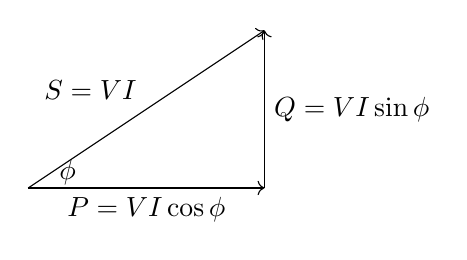
\begin{tikzpicture}
    \draw[->] (0,0) -- (3,0) node[midway, below] {$P = VI \cos\phi$};
    \draw[->] (3,0) -- (3,2) node[midway, right] {$Q = VI \sin\phi$};
    \draw[->] (0,0) -- (3,2) node[midway, above left] {$S = VI$};
    \node at (0.5, 0.2) {$\phi$};
\end{tikzpicture}
\captionof{figure}{Power Triangle}
\end{center}

\textbf{Significance:}
\begin{itemize}
    \item \keyword{Active power}: Does useful work
    \item \keyword{Reactive power}: Maintains fields
    \item \keyword{Power factor}: Efficiency indicator ($P/S$)
\end{itemize}
\end{solutionbox}

\begin{mnemonicbox}
\mnemonic{"Power Triangle: Please Qualify Students" (P, Q, S components)}
\end{mnemonicbox}

\questionmarks{5(c OR)}{7}{Explain wiring of lamp control from one place and staircase type.}

\begin{solutionbox}
\textbf{Answer:}

\textbf{1. Lamp Control from One Place:}

\textbf{Circuit Diagram:}
\begin{center}
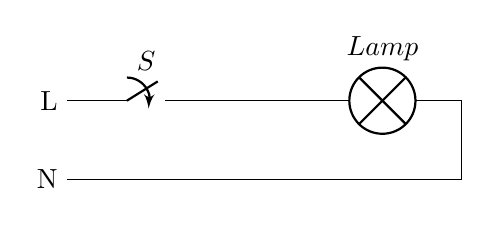
\begin{tikzpicture}
    \draw (0,0) node[left]{L} to[switch, l=$S$] (2,0) -- (3,0) to[lamp, l=$Lamp$] (5,0) -- (5,-1) -- (0,-1) node[left]{N};
\end{tikzpicture}
\captionof{figure}{One-way Control}
\end{center}

\textbf{Components:}
\begin{itemize}
    \item \textbf{SPST Switch}: Single pole, single throw
    \item \textbf{Live wire control}: Switch in live wire for safety
\end{itemize}

\textbf{2. Staircase Wiring (Two-Way Control):}

\textbf{Circuit Diagram:}
\begin{center}
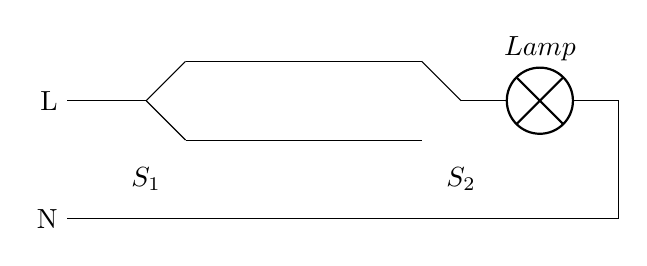
\begin{tikzpicture}
    \draw (0,0) node[left]{L} -- (1,0);
    
    % Switch 1 (SPDT)
    \draw (1,0) -- (1.5, 0.5) coordinate (S1A);
    \draw (1,0) -- (1.5, -0.5) coordinate (S1B);
    \node at (1,-1) {$S_1$};
    
    % Strappers
    \draw (1.5, 0.5) -- (4.5, 0.5);
    \draw (1.5, -0.5) -- (4.5, -0.5);
    
    % Switch 2 (SPDT)
    \coordinate (S2A) at (4.5, 0.5);
    \coordinate (S2B) at (4.5, -0.5);
    \draw (S2A) -- (5,0); % Connected to top for illustration
    \node at (5,-1) {$S_2$};
    
    % Lamp
    \draw (5,0) to[lamp, l=$Lamp$] (7,0) -- (7,-1.5) -- (0,-1.5) node[left]{N};
\end{tikzpicture}
\captionof{figure}{Two-way Staircase Wiring}
\end{center}

\textbf{Switch Positions:}
\begin{center}
\captionof{table}{Staircase Logic}
\begin{tabulary}{\linewidth}{|L|L|L|}
\hline
\textbf{S1 Position} & \textbf{S2 Position} & \textbf{Lamp Status} \\ \hline
Up & Up & ON \\ \hline
Up & Down & OFF \\ \hline
Down & Up & OFF \\ \hline
Down & Down & ON \\ \hline
\end{tabulary}
\end{center}

\textbf{Applications:}
\begin{itemize}
    \item \keyword{Staircase lighting}: Control from top and bottom
    \item \keyword{Long corridors}: Control from both ends
    \item \keyword{Bedroom lighting}: Control from bed and door
\end{itemize}
\end{solutionbox}

\begin{mnemonicbox}
\mnemonic{"Two-way Toggles, Two places" (Two switches, two locations)}
\end{mnemonicbox}

\end{document}
